\documentclass[a4paper]{article}

%% Language and font encodings
\usepackage[english]{babel}
\usepackage[utf8x]{inputenc}
\usepackage[T1]{fontenc}

%% Sets page size and margins
\usepackage[a4paper,top=3cm,bottom=2cm,left=3cm,right=3cm,marginparwidth=1.75cm]{geometry}

%% Useful packages
\usepackage{amsmath}
\usepackage{graphicx}
\usepackage[colorinlistoftodos]{todonotes}
\usepackage[colorlinks=true, allcolors=blue]{hyperref}

\title{Assignment Reinforcement Learning}
\author{Alexandra Bremers \and Renate van der Bent}

\begin{document}
\maketitle

\section{Introduction: skating problem}
In this assignment, we implemented a population of skaters skating on the surface of a torus. In order to successfully coordinate among other skaters, the skaters must learn to avoid collisions. To avoid collisions, they must learn in which direction to move. The skaters learn to avoid collision by reinforcement learning. They learn by receiving rewards for avoiding collision, and getting punished in case they cause a collision. The skaters will then try to take actions, i.e. choose directions to move in, to maximize their reward. We chose to implement this skater model in Python. Collision avoiding behaviour can be found in many multi-agent systems. For example, it can also be seen in flocking behaviour, where birds try to stay close together but at the same time need to avoid collision. Another example where agents need to coordinate their directions to avoid collision is in aircraft, where planes need to be carefully manoeuvered. However, these systems do not typically involve (explicit) reinforcement learning. Reinforcement Learning is a type of machine learning based on maximizing reward, and is very suitable to our skating problem. 

\section{Approach}
We built a model of the simplified problem in Python (version  3.6) with use of the Mesa library [1] and executed in an interactive Jupyter Notebook [2]. 
The environment in the model consists of a toroidal grid space of height h and width w. The grid does not limit the maximum allowed number of agents in a cell. For a single agent, we can visualize a hypothetical scenario in a grid, corresponding with the illustration of a Von Neumann neighborhood in Fig. 1.  

\begin{figure}[h]
\makebox[\textwidth][c]{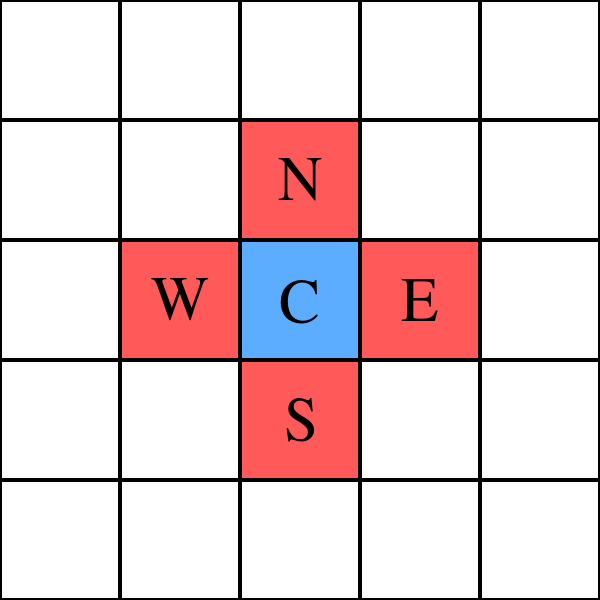
\includegraphics[width=0.3\textwidth]{neumann.png}}
\caption{Von Neumann neighborhood. Source: Wikimedia Commons}
\end{figure}
In this example we could imagine an agent with location (2,2) in a 5x5 grid where both axes go from 0 to 4. The agent has four Von Neumann neighbors, namely at his North (2,1), West (1,2), East (3,2) and South (2,3). The possible steps for the agent to take are these four neighboring cells, making the angle resolution k having a fixed value of 90 (degrees). The motivation behind the choice for a Von Neumann neighborhood as opposed to a Moore neighborhood is that the Moore neighborhood, although allowing for a lower angle resolution, contains inconsistencies when a radius is considered. For the neighbors in the Von Neumann neighborhood in a square grid, the cell-center to cell-center radius is equal to the length and width of a single cell, say c.  This, however, does not hold for the diagonal neighbors in the Moore neighborhood: in that case the cell-center to cell-center distance can be calculated by the Pythagorean Theorem and is given by $\sqrt[]{2c^2}$. By choosing the Von Neumann neighborhood as the basis for our model, we arrive at a simplified implementation of the skater problem with a fixed angle resolution of 90 degrees and a fixed radius of c.
\newline

We create a number of N agents, each with attributes to store their number of collisions, previously headed direction and reward values for each angle. The angle is determined by the angle between the direction of the new position (north, west, east or south) and the direction that the agent considered in the previous round. With every step, one of the agents considers a possible new location among its neighboring cells, with a certain angle from the direction it was headed previously. When the cell is already occupied by another agent, the agent receives a reward R2 and does not move this turn. If however the cell is not occupied, the agent moves to the cell and receives a reward R1. The goal of each agent is to aim for a reward as high as possible by keeping track of the previous rewards that choices for certain angles resulted in, and choosing an angle for a new action based on reinforcement learning. 

The type of reinforcement learning used is $\epsilon$-greedy. $\epsilon$-greedy is an algorithm that is commonly mentioned and used in literature on the multi-armed bandit problem. In essence there are two possible behaviors for the agent: exploiting and exploring. The parameter given by $\epsilon$ describes the probability that the agent explores, while in all other cases, given by $1-\epsilon$, the agent will exploit. By exploitation is meant that the agent will choose the action (angle) that in previous rounds resulted in the highest cumulative reward. By exploration however, a new action is randomly chosen from the possible actions.

\section{Results}
Firstly we study a scenario where collision is heavily punished and $\epsilon$ is relatively small. We consider a grid with h = 50, w = 50, R1 = 2, R2 = -250 and $\epsilon$ = 0.1. With a small sized population of 40 agents (spread across 2500 cells), the development of the average reward for each angle through 10000 steps is given in Fig. 2.
\begin{figure}[h]
\makebox[\textwidth][c]{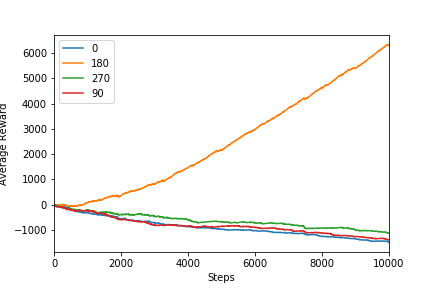
\includegraphics[width=0.7\textwidth]{fig2.png}}
\caption{N = 40, $\epsilon$ = 0.1, steps = 10000, h = w = 50, R1 = 2, R2 = -250} 
\end{figure}
With these settings, something interesting is happening. Due to the lower $\epsilon$-value, the agent will stick with a 90 percent chance to a successful move. Because the agent population is not dense, the likelihood that the agent collides is low. If that happens however, the reward for the angle in question drops by 250, a value that can only be corrected with 125 occurrences of exploration resulting in that move and also not resulting in another collision. We see however that the reward of 180 degrees developed slowly in the beginning, until the other angles lost a lot of reward. A feedback loop emerged where all the agents chose for the 180 degree angle move within exploitation, with an occasional exploration leading to a slight growth or drop in reward for other angles. Because of the large numbers on the x-axis the peaks are not very visible, however, if we take a look at Fig. 3 we see a run of the model with the same configuration, only with 500 steps in stead of 10000, which clearly shows the peaks.
\newline

\begin{figure}[h]
\makebox[\textwidth][c]{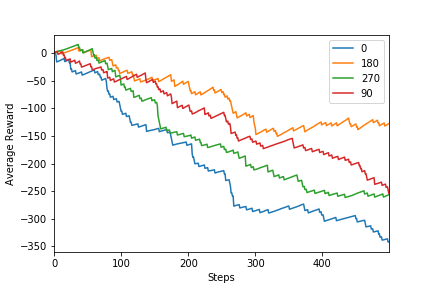
\includegraphics[width=0.7\textwidth]{fig3.png}}
\caption{N = 40, $\epsilon$ = 0.1, steps = 500, h = w = 50, R1 = 2, R2 = -250} 
\end{figure}

If we, however, plot the same model with a smaller N to space ratio of N = 40, but h = 20, w = 20 (so, 40 agents in 400 cells), we see something different happening in Fig. 4. It seems that since the chance of collision is a lot higher, there is no angle that has a much higher reward than others, leading to no reinforcing behavior. 

\begin{figure}[h]
\makebox[\textwidth][c]{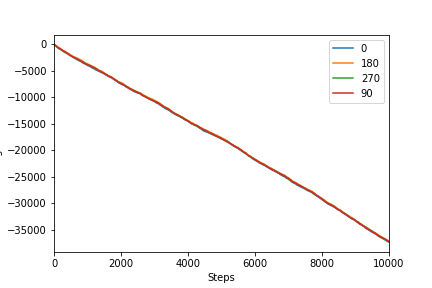
\includegraphics[width=0.7\textwidth]{fig4.png}}
\caption{N = 40, $\epsilon$ = 0.1, steps = 1000, h = w = 20, R1 = 2, R2 = -250} 
\end{figure}

For our second scenario we are going to assume a model with the same configurations as above, except that $\epsilon$ will be set to a higher value of 0.45, leading to more exploration. We see that the graph looks similar to Fig.2, but the average reward for the winning strategy after 10000 steps is lower.

\begin{figure}[h]
\makebox[\textwidth][c]{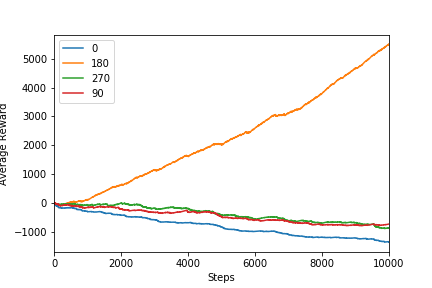
\includegraphics[width=0.7\textwidth]{fig5.png}}
\caption{N = 40, $\epsilon$ = 0.45, steps = 1000, h = w = 20, R1 = 2, R2 = -250} 
\end{figure}

\pagebreak

\section{Answers to theoretical questions}
Although it may seem like the N skaters converge to one angle, this is not always the case. As we have seen in Fig.4, when the reward (or "punishment") R2 for a collision is a large negative number and the population is dense, we see that no convergence happens. An explanation for this is that exploitation barely has an effect. When one angle has a slightly higher cumulative reward and gets chosen, there is a big chance that the reward immediately drops through collision, or the reward may go up by a very small number. We can say that in this scenario reinforcement learning does not help find a solution and the skaters cannot reach an optimal reward value. From this we can conclude that convergence does not happen at all times.

But apart from those conditions, in normal conditions it is almost surely the case that convergence happens to the angle of 180 degrees. This can be explained if we look at the neighbors involved.

\begin{figure}[h]
\makebox[\textwidth][c]{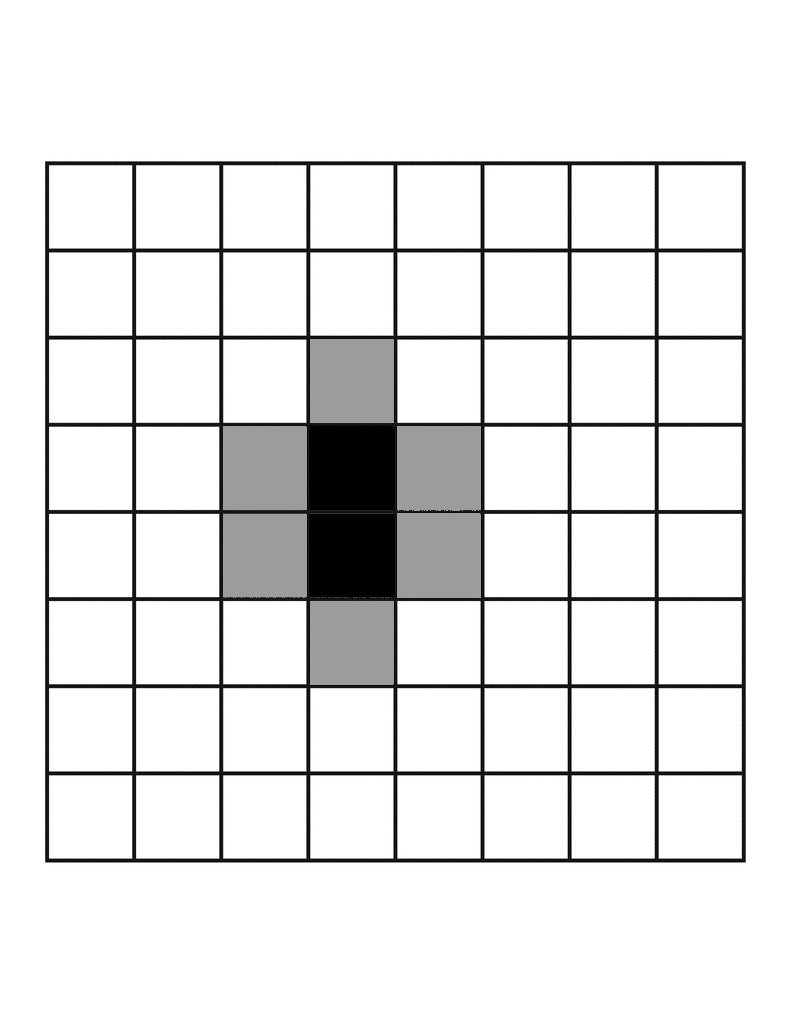
\includegraphics[width=0.18\textwidth]{grid180.png}}
\caption{Location cells (black) and neighbor cells (grey) for an agent that always chooses an angle of 180 degrees. We see 2 location cells involved.} 
\end{figure}

\begin{figure}[h]
\makebox[\textwidth][c]{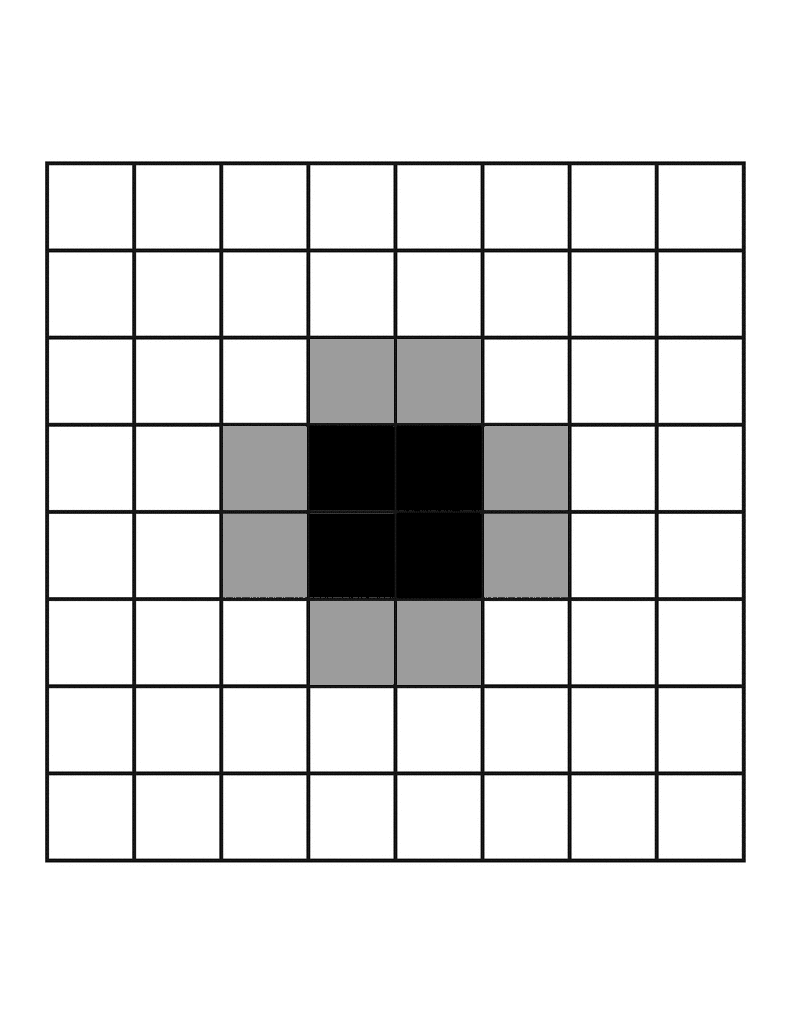
\includegraphics[width=0.18\textwidth]{grid90270.png}}
\caption{Location cells (black) and neighbor cells (grey) for an agent that always chooses an angle of 90 or 270 degrees. We see 4 location cells involved.} 
\end{figure}

\begin{figure}[h]
\makebox[\textwidth][c]{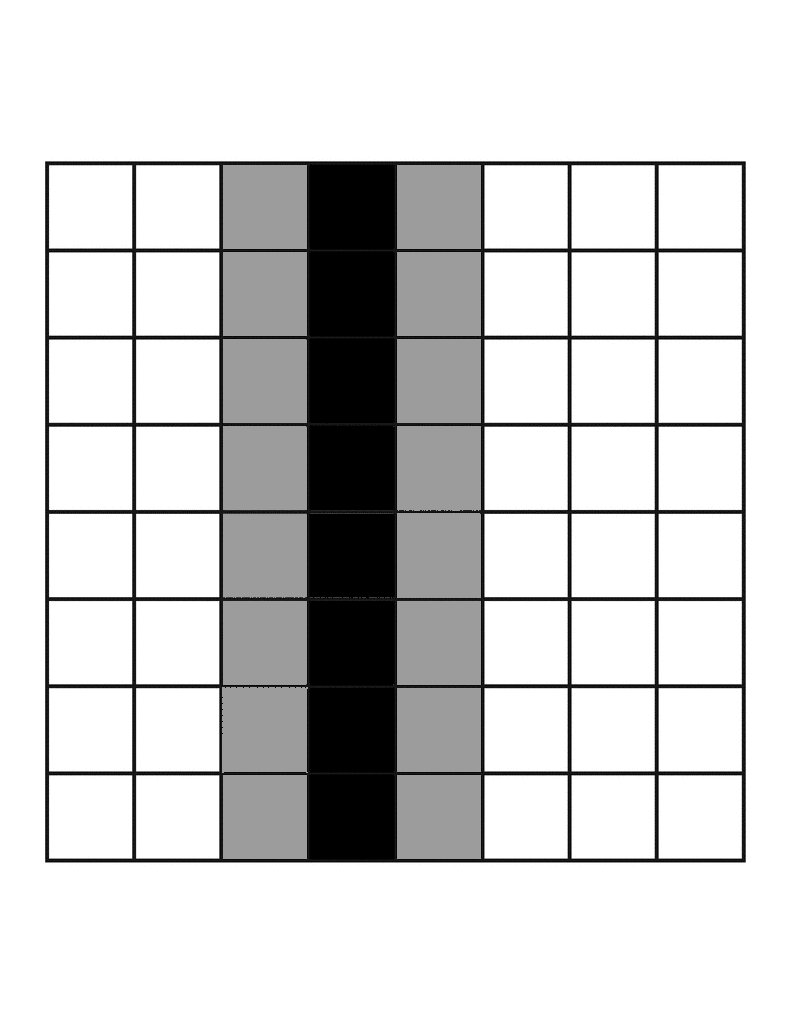
\includegraphics[width=0.18\textwidth]{grid0.png}}
\caption{Location cells (black) and neighbor cells (grey) for an agent that always chooses an angle of 0 degrees. The number of location cells is h (w if headed horizontally).} 
\end{figure}

We see from Fig. 6, Fig.7 and Fig.8 different scenarios of an agent choosing a certain angle at all times in a 8 X 8 grid. An agent always choosing an angle of 180 degrees only moves between two grid cells at all times. The chance that one of its location cells is going to be occupied, leading to a collision, is smaller than in cases where there are more location cells involved, which leads to a higher reward over time.
If the height becomes 2 or 1, the graphs for 180 degrees and 0 degrees would look the same when the agents are headed in the (vertical) direction depicted on the figures. In that case a conversion towards 0 degrees would be equally likely as a conversion to 180 degrees. Since this is not a very likely scenario we can state that it is almost surely the case that the N skaters converge to 180 degrees in this model.

\bibliographystyle{alpha}
\bibliography{sample}


[1] Masad et al. (2015). Mesa: An Agent-Based Modeling Framework. PROC. OF THE 14th PYTHON IN SCIENCE CONF. (SCIPY 2015), p53-60.
\newline

[2] Jupyter Notebook, see http://www.jupyter.com/
\newline

[3] Model code depository: see 
\newline
\url{https://github.com/awdbremers/MAA_AlexandraRenate_RLEGCollisionModel}
\newline
\end{document}